\documentclass{article}

%other packages
\usepackage[a4paper]{geometry}
\setlength\parindent{0pt}

%maths
\usepackage{mathtools}
\usepackage{amsmath}
\usepackage{amssymb}
\usepackage{amsfonts}
\usepackage{autobreak}

%tikzpicture
\usepackage{tikz}
\usepackage{scalerel}
\usepackage{pict2e}
\usepackage{tkz-euclide}
\usepackage{tikz-3dplot}
\usetikzlibrary{calc}
\usetikzlibrary{patterns,arrows.meta}
\usetikzlibrary{shadows}
\usetikzlibrary{external}
\usetikzlibrary{decorations.pathreplacing,angles,quotes}
\usetikzlibrary{perspective,spath3}

%pgfplots
\usepackage{pgfplots}
\pgfplotsset{compat=1.18}
\usepgfplotslibrary{statistics}
\usepgfplotslibrary{fillbetween}

\pgfplotsset{
    standard/.style={
    axis line style = thick,
    trig format=rad,
    enlargelimits,
    axis x line=middle,
    axis y line=middle,
    enlarge x limits=0.15,
    enlarge y limits=0.15,
    every axis x label/.style={at={(currenot axis.right of origin)},anchor=north west},
    every axis y label/.style={at={(current axis.above origin)},anchor=south east}
    }
}

\begin{document}

The Parabola.
\hrule

\begin{center}
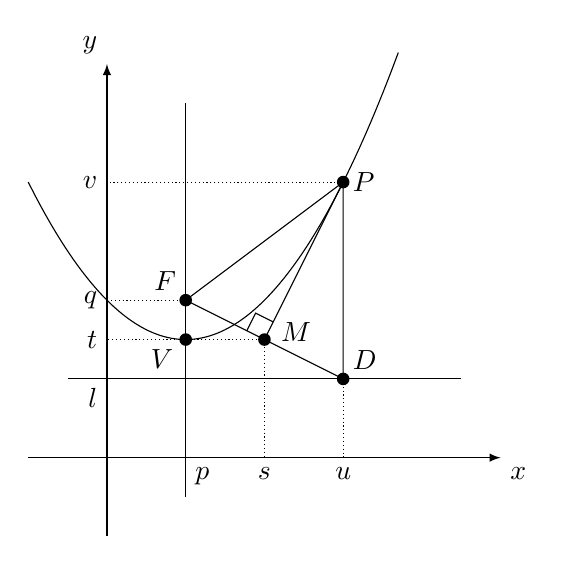
\begin{tikzpicture}[]
%%% COORDINATES %%%
\coordinate (F) at (1,2); % focus
\coordinate (D) at (3,1); % diameter
\coordinate (M) at (2,1.5); % midpoint
\coordinate (P) at (3,3.5); % point on parabola
\coordinate (V) at (1,1.5); % vertex
\fill[] (F) circle [radius=0.08] node[above left]{$F$};
\fill[] (D) circle [radius=0.08] node[above right]{$D$};
\fill[] (M) circle [radius=0.08];
\node at (2.4,1.6) {$M$};
\fill[] (V) circle [radius=0.08];
\node at (0.7,1.25) {$V$};
\fill[] (P) circle [radius=0.08] node[right]{$P$};

%%% AXES %%%
\draw[-latex] (-1,0) -- (5,0) node[pos=1,below right] {$x$};
\draw[-latex] (0,-1) -- (0,5) node[pos=1,above left] {$y$};

%%% TRIANGLE %%%
\draw[] (P) -- (M) -- (F) -- (D) -- (P) -- (F) -- cycle;
\draw pic[draw,-,angle eccentricity=1.4, angle radius=0.25cm]{right angle=F--M--P};

%%% DOTTED LINES %%%
% horizontal lines
\draw[thin,densely dotted] (F) -| (0,0);
\draw[thin,densely dotted] (M) -| (0,0);
\draw[thin,densely dotted] (P) -| (0,0);
\node[left] at (0,2) {$q$};
\node[left] at (0,1.5) {$t$};
\node[left] at (0,3.5) {$v$};
\node[below left] at (0,1) {$l$};
% vertical lines
\draw[thin,densely dotted] (F) |- (0,0);
\draw[thin,densely dotted] (M) |- (0,0);
\draw[thin,densely dotted] (D) |- (0,0);
\node[below right] at (1,0) {$p$};
\node[below] at (2,0) {$s$};
\node[below] at (3,0) {$u$};

%%% CONSTRUCTIONS %%%
\draw[] (-0.5,1) -- (4.5,1);
\draw[] (1,-0.5) -- (1,4.5);




%%% THE PARABOLA %%%
\draw[domain=-1:3.7,smooth,variable=\u,samples=50]
  plot ({\u},{0.5*\u*\u-\u+2});
\end{tikzpicture}
\end{center}

Focus: $F$

Directrix: $y=l$

Diamater: $x=u$

Axis: $x=p$

Vertex: $V$

Tangent: $\tau$

Normal: $\nu$

\[\Rightarrow M=(s,t)=\left(\frac{p+u}{2},\frac{q+l}{2}\right)\]
\[\Rightarrow\mbox{slope}(FD)=\frac{\Delta y}{\Delta x}=\frac{l-q}{u-p}\]
\[\Rightarrow\mbox{slope}(MP)=\frac{-1}{\mbox{slope}(FD)}=\frac{p-u}{l-q}\]
\[\Rightarrow\mbox{line}(MP)=f(x)=mx+b\Rightarrow\frac{q+l}{2}=\frac{p-u}{l-q}\cdot\frac{p+u}{2}+b\Rightarrow b=\frac{l^2-q^2-p^2+u^2}{2(l-q)}\]
\[\therefore f(u)=\frac{2up-u^2+l^2-q^2-p^2}{2(l-q)}\]


\end{document}